\ifdefined\COMPLETE
\else
\documentclass[12pt]{article}
\usepackage{tikz}
\usetikzlibrary{shapes, calc, arrows, through, intersections, decorations.pathreplacing, patterns}

\begin{document}
\fi

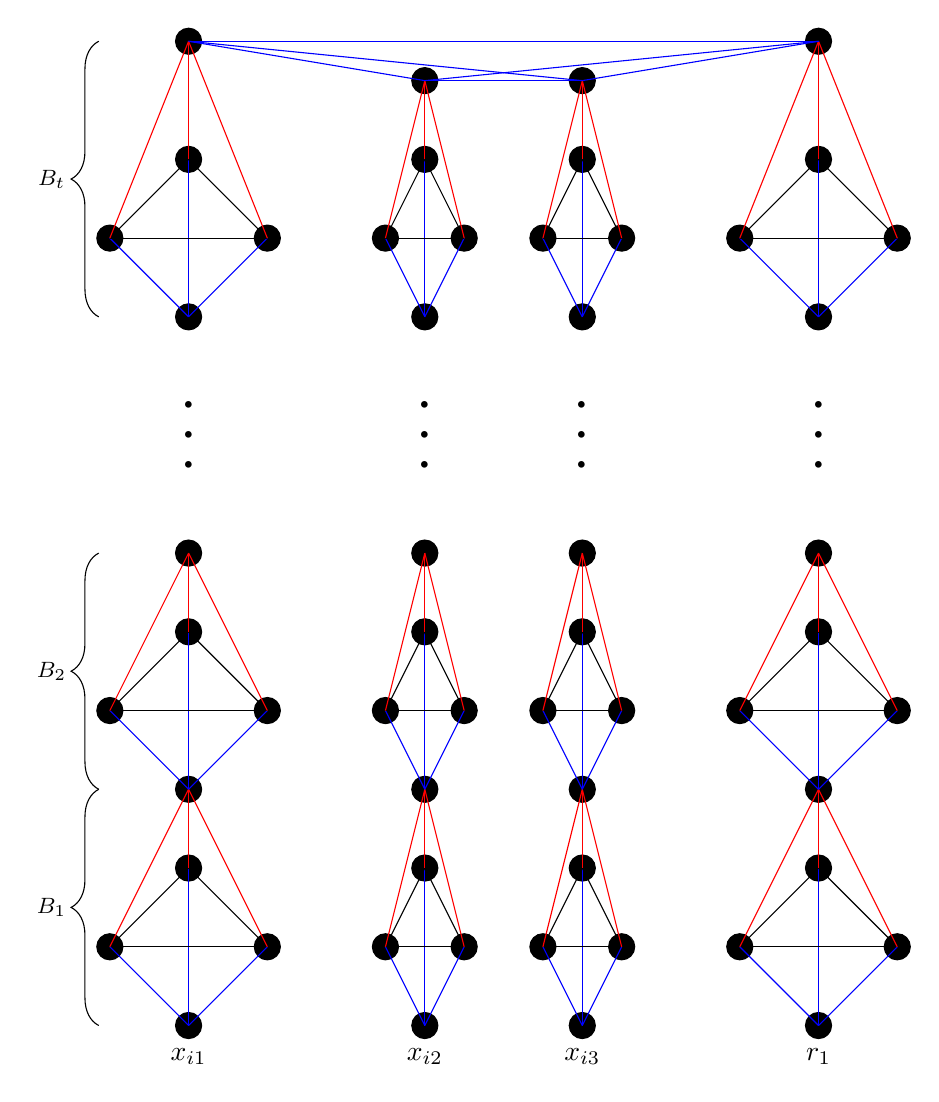
\begin{tikzpicture}
	  \node[circle,draw,minimum size=1mm,,fill=black,label=below:$x_{i1}$] at (0, 0){};
	  \node[circle,draw,fill=black] at (0, 2){};
	  \node[circle,draw,fill=black] at (-1, 1){};
	  \node[circle,draw,fill=black] at (1, 1){};
	  \node[circle,draw,fill=black] at (0, 3){};

	  \node[circle,draw,fill=black] at (0, 5){};
	  \node[circle,draw,fill=black] at (-1, 4){};
	  \node[circle,draw,fill=black] at (1, 4){};
	  \node[circle,draw,fill=black] at (0, 6){};
			
	  \node[circle,draw,fill=black] at (0, 9){};
	  \node[circle,draw,fill=black] at (0, 11){};
	  \node[circle,draw,fill=black] at (-1, 10){};
	  \node[circle,draw,fill=black] at (1, 10){};
	  \node[circle,draw,fill=black] at (0, 12.5){};
	
	  \draw[blue] (0, 0) -- (0, 2);
	  \draw[blue] (0, 0) -- (-1, 1);
	  \draw[blue] (0, 0) -- (1, 1);
	  \draw (1, 1) -- (-1, 1);
	  \draw (1, 1) -- (0, 2);
	  \draw (-1, 1) -- (0, 2);
	  \draw[red] (1, 1) -- (0, 3);
	  \draw[red] (-1, 1) -- (0, 3);
	  \draw[red] (0, 3) -- (0, 2);
		
	  \draw[blue] (0, 3) -- (0, 5);
	  \draw[blue] (0, 3) -- (-1, 4);
	  \draw[blue] (0, 3) -- (1, 4);
	  \draw (1, 4) -- (-1, 4);
	  \draw (1, 4) -- (0, 5);
	  \draw (-1, 4) -- (0, 5);
	  \draw[red] (1, 4) -- (0, 6);
	  \draw[red] (-1, 4) -- (0, 6);
	  \draw[red] (0, 6) -- (0, 5);
	
	  \draw[blue] (0, 9) -- (0, 11);
	  \draw[blue] (0, 9) -- (-1, 10);
	  \draw[blue] (0, 9) -- (1, 10);
	  \draw (1, 10) -- (-1, 10);
	  \draw (1, 10) -- (0, 11);
	  \draw (-1, 10) -- (0, 11);
	  \draw[red] (1, 10) -- (0, 12.5);
	  \draw[red] (-1, 10) -- (0, 12.5);
	  \draw[red] (0, 12.5) -- (0, 11);
	  	
	  \node[circle,draw,minimum size=1mm,,fill=black,label=below:$x_{i2}$] at (3, 0){};
	  \node[circle,draw,fill=black] at (3, 2){};
	  \node[circle,draw,fill=black] at (2.5, 1){};
	  \node[circle,draw,fill=black] at (3.5, 1){};
	  \node[circle,draw,fill=black] at (3, 3){};
	
	  \node[circle,draw,fill=black] at (3, 5){};
	  \node[circle,draw,fill=black] at (2.5, 4){};
	  \node[circle,draw,fill=black] at (3.5, 4){};
	  \node[circle,draw,fill=black] at (3, 6){};
		
	  \node[circle,draw,fill=black] at (3, 9){};
	  \node[circle,draw,fill=black] at (3, 11){};
	  \node[circle,draw,fill=black] at (2.5, 10){};
	  \node[circle,draw,fill=black] at (3.5, 10){};
	  \node[circle,draw,fill=black] at (3, 12){};
	  		
	  \draw[blue] (3, 0) -- (3, 2);
	  \draw[blue] (3, 0) -- (2.5, 1);
	  \draw[blue] (3, 0) -- (3.5, 1);
	  \draw (3.5, 1) -- (2.5, 1);
	  \draw (3.5, 1) -- (3, 2);
	  \draw (2.5, 1) -- (3, 2);
	  \draw[red] (2.5, 1) -- (3, 3);
	  \draw[red] (3.5, 1) -- (3, 3);
	  \draw[red] (3, 3) -- (3, 2);
	  
	  \draw[blue] (3, 3) -- (3, 5);
	  \draw[blue] (3, 3) -- (2.5, 4);
	  \draw[blue] (3, 3) -- (3.5, 4);
	  \draw (3.5, 4) -- (2.5, 4);
	  \draw (3.5, 4) -- (3, 5);
	  \draw (2.5, 4) -- (3, 5);
	  \draw[red] (3.5, 4) -- (3, 6);
	  \draw[red] (2.5, 4) -- (3, 6);
	  \draw[red] (3, 6) -- (3, 5);
	  
	  \draw[blue] (3, 9) -- (3, 11);
	  \draw[blue] (3, 9) -- (2.5, 10);
	  \draw[blue] (3, 9) -- (3.5, 10);
	  \draw (3.5, 10) -- (2.5, 10);
	  \draw (3.5, 10) -- (3, 11);
	  \draw (2.5, 10) -- (3, 11);
	  \draw[red] (3.5, 10) -- (3, 12);
	  \draw[red] (2.5, 10) -- (3, 12);
	  \draw[red] (3, 12) -- (3, 11);
	  
	  \node[circle,draw,minimum size=1mm,,fill=black,label=below:$x_{i3}$] at (5, 0){};
	  \node[circle,draw,fill=black] at (5, 2){};
	  \node[circle,draw,fill=black] at (4.5, 1){};
	  \node[circle,draw,fill=black] at (5.5, 1){};
	  \node[circle,draw,fill=black] at (5, 3){};
	
	  \node[circle,draw,fill=black] at (5, 5){};
	  \node[circle,draw,fill=black] at (4.5, 4){};
	  \node[circle,draw,fill=black] at (5.5, 4){};
	  \node[circle,draw,fill=black] at (5, 6){};
		
	  \node[circle,draw,fill=black] at (5, 9){};
	  \node[circle,draw,fill=black] at (5, 11){};
	  \node[circle,draw,fill=black] at (4.5, 10){};
	  \node[circle,draw,fill=black] at (5.5, 10){};
	  \node[circle,draw,fill=black] at (5, 12){};
	  		
	  \draw[blue] (5, 0) -- (5, 2);
	  \draw[blue] (5, 0) -- (4.5, 1);
	  \draw[blue] (5, 0) -- (5.5, 1);
	  \draw (5.5, 1) -- (4.5, 1);
	  \draw (5.5, 1) -- (5, 2);
	  \draw (4.5, 1) -- (5, 2);
	  \draw[red] (5.5, 1) -- (5, 3);
	  \draw[red] (4.5, 1) -- (5, 3);
	  \draw[red] (5, 3) -- (5, 2);
	  
	  \draw[blue] (5, 3) -- (5, 5);
	  \draw[blue] (5, 3) -- (4.5, 4);
	  \draw[blue] (5, 3) -- (5.5, 4);
	  \draw (5.5, 4) -- (4.5, 4);
	  \draw (5.5, 4) -- (5, 5);
	  \draw (4.5, 4) -- (5, 5);
	  \draw[red] (5.5, 4) -- (5, 6);
	  \draw[red] (4.5, 4) -- (5, 6);
	  \draw[red] (5, 6) -- (5, 5);
	  
	  \draw[blue] (5, 9) -- (5, 11);
	  \draw[blue] (5, 9) -- (4.5, 10);
	  \draw[blue] (5, 9) -- (5.5, 10);
	  \draw (5.5, 10) -- (4.5, 10);
	  \draw (5.5, 10) -- (5, 11);
	  \draw (4.5, 10) -- (5, 11);
	  \draw[red] (5.5, 10) -- (5, 12);
	  \draw[red] (4.5, 10) -- (5, 12);
	  \draw[red] (5, 12) -- (5, 11);
	  
	  \node[circle,draw,minimum size=1mm,label=below:$r_{1}$,fill=black] at (8, 0){};
	  \node[circle,draw,fill=black] at (8, 2){};
	  \node[circle,draw,fill=black] at (7, 1){};
	  \node[circle,draw,fill=black] at (9, 1){};
	  \node[circle,draw,fill=black] at (8, 3){};

	  \node[circle,draw,fill=black] at (8, 5){};
	  \node[circle,draw,fill=black] at (7, 4){};
	  \node[circle,draw,fill=black] at (9, 4){};
	  \node[circle,draw,fill=black] at (8, 6){};
			
	  \node[circle,draw,fill=black] at (8, 9){};
	  \node[circle,draw,fill=black] at (8, 11){};
	  \node[circle,draw,fill=black] at (7, 10){};
	  \node[circle,draw,fill=black] at (9, 10){};
	  \node[circle,draw,fill=black] at (8, 12.5){};
	
	  \draw[blue] (8, 0) -- (8, 2);
	  \draw[blue] (8, 0) -- (7, 1);
	  \draw[blue] (8, 0) -- (9, 1);
	  \draw (9, 1) -- (7, 1);
	  \draw (9, 1) -- (8, 2);
	  \draw (7, 1) -- (8, 2);
	  \draw[red] (9, 1) -- (8, 3);
	  \draw[red] (7, 1) -- (8, 3);
	  \draw[red] (8, 3) -- (8, 2);
		
	  \draw[blue] (8, 3) -- (8, 5);
	  \draw[blue] (8, 3) -- (7, 4);
	  \draw[blue] (8, 3) -- (9, 4);
	  \draw (9, 4) -- (7, 4);
	  \draw (9, 4) -- (8, 5);
	  \draw (7, 4) -- (8, 5);
	  \draw[red] (9, 4) -- (8, 6);
	  \draw[red] (7, 4) -- (8, 6);
	  \draw[red] (8, 6) -- (8, 5);
	
	  \draw[blue] (8, 9) -- (8, 11);
	  \draw[blue] (8, 9) -- (7, 10);
	  \draw[blue] (8, 9) -- (9, 10);
	  \draw (9, 10) -- (7, 10);
	  \draw (9, 10) -- (8, 11);
	  \draw (7, 10) -- (8, 11);
	  \draw[red] (9, 10) -- (8, 12.5);
	  \draw[red] (7, 10) -- (8, 12.5);
	  \draw[red] (8, 12.5) -- (8, 11);
	
	  \draw[blue] (0, 12.5) -- (8, 12.5);
	  \draw[blue] (0, 12.5) -- (5, 12);
	  \draw[blue] (0, 12.5) -- (3, 12);
	  \draw[blue] (3, 12) -- (5, 12);
	  \draw[blue] (3, 12) -- (8, 12.5);
	  \draw[blue] (5, 12) -- (8, 12.5);
	  
	  \path (0, 9) -- (0, 6) node [black, font=\Huge, midway, sloped] {$\dots$};
	  \path (3, 9) -- (3, 6) node [black, font=\Huge, midway, sloped] {$\dots$};
	  \path (5, 9) -- (5, 6) node [black, font=\Huge, midway, sloped] {$\dots$};
	  \path (8, 9) -- (8, 6) node [black, font=\Huge, midway, sloped] {$\dots$};
	  
	  \draw [decorate,decoration={brace,amplitude=10pt},xshift=-4pt,yshift=0pt]
(-1,0) -- (-1,3) node [black,midway,xshift=-0.6cm] 
{\footnotesize $B_1$};
	  \draw [decorate,decoration={brace,amplitude=10pt},xshift=-4pt,yshift=0pt]
(-1,3) -- (-1,6) node [black,midway,xshift=-0.6cm] 
{\footnotesize $B_2$};
	  \draw [decorate,decoration={brace,amplitude=10pt},xshift=-4pt,yshift=0pt]
(-1,9) -- (-1,12.5) node [black,midway,xshift=-0.6cm] 
{\footnotesize $B_t$};

\end{tikzpicture}

\ifdefined\COMPLETE
\else
\end{document}
\fi
